\documentclass[oneside, final, 12pt, a4paper]{article}
\usepackage[utf8]{inputenc}
\usepackage[T2A]{fontenc}
\usepackage[english, russian]{babel}
\usepackage{vmargin}
\usepackage{amsthm,amsfonts,amsmath,amssymb,amscd}
\usepackage{xcolor}
\usepackage{hyperref}
\usepackage{indentfirst}
\usepackage{color}
\usepackage{listings} 
\usepackage{caption}
\usepackage{graphicx}
\usepackage{hyperref}
\usepackage{cite}
\usepackage{psfrag}
\usepackage[top=2cm,bottom=2cm,left=2.5cm,right=1cm]{geometry}
% \setpapersize{A4}
\setmarginsrb{2cm}{1.5cm}{1cm}{1.5cm}{0pt}{0mm}{0pt}{13mm}
\linespread{1.3}

\DeclareCaptionFont{white}{\color{white}}

\DeclareCaptionFormat{listing}{\colorbox{gray}{\parbox{\textwidth}{#1#2#3}}}
% \captionsetup[lstlisting]{format=listing,labelfont=white,textfont=white}

\newenvironment{compactlist}{
    \begin{list}{{$\bullet$}}{
        \setlength\partopsep{0pt}
        \setlength\parskip{0pt}
        \setlength\parsep{0pt}
        \setlength\topsep{0pt}
        \setlength\itemsep{0pt}
    }
}{
    \end{list}
}

\begin{document}

\begin{titlepage}

\begin{center}
  
\includegraphics[width=8cm, height=4cm]{img/msu_logo.jpg}
\end{center}

\begin{center}
Московский государственный университет имени М.В. Ломоносова\\
\vspace{0.1 cm}
Факультет вычислительной математики и кибернетики\\
\vspace{0.1 cm}
Кафедра математической статистики

\vspace{3cm}
{\Large Новиков Дмитрий Александрович }\\
\vspace{1cm}

{\bf\LARGE Сравнение трех моделей ценообразования опционов}\\ \vspace{2cm}
ВЫПУСКНАЯ КВАЛИФИКАЦИОННАЯ РАБОТА

\end{center}
\vspace{2cm}
\begin{flushright}

{\bf Научный руководитель:}\\
к.ф.-м.н.\\
Л.\,В. Назаров

\end{flushright}

 \vspace{4.5cm}

\centerline {Москва, 2018}
\end{titlepage}

\newpage
\tableofcontents

\newpage
\large
\leftline{\bf Список обозначений}
\leftline{\hrulefill}
\vskip0.25cm
\normalfont

Далее будут использованы следующие обозначения:\\
$\mathbb{E}\xi$~-- математическое ожидание с.в. $\xi$\\
$\mathbb{D}\xi$~-- дисперсия с.в. $\xi$\\
$\displaystyle \Phi(x)=\frac{1}{\sqrt{2\pi}}\int\limits_{-\infty}^{x}e^{-\frac{t^2}{2}}\,dt$~-- ф.р. стандартной нормальной с.в. \( \xi \sim \mathcal{N}(0, 1)\) \\
$W_t$~-- винеровский процесс\\
$S_t$~-- спот, рыночная цена базового актива на момент времени $t$. $S_0$ - текущая цена\\
$r$~-- безрисковая процентная ставка с непрерывным начислением\\
$q$~-- дивиденды с непрерывным начислением\\
$T$~-- время до погашения опциона\\
$K$~-- страйк, договорная цена базового актива\\
$C$~-- цена европейского колл-опциона\\
$P$~-- цена европейского пут-опциона\\
$c$~-- логарифм цены европейского колл-опциона

% Введение
\newpage
\section{Цель работы}
На данный момент существует множество разнообразных моделей ценообразования опционов, но они редко сравниваются между собой, кроме разве что модели Блэка-Шоулза, которая считается отправной точкой при описании почти любой новой модели оценки стоимости опционов. Ввиду очевидного несоответствия условий применимости модели Блэка-Шоулза к реальныи биржевым процессам (например, предполагаемое постоянство волатильности и процентной ставки), такие сравнения заведомо слабо информативны в отношении качества модели. \par

Цель настоящей работы состоит в проведении сравнительного анализа трех моделей определения цены опциона: Хестона, Variance Gamma и Finite Moment Log Stable. Сравниваются скорость калибровки параметров моделей, качество калибровки, качество прогнозирования, устойчивость откалиброванных параметров по времени. В кодовой реализации моделей используется подход, предложенный Карром (Peter Carr) и Маданом (Dilip B. Madan) в статье <<Option pricing using the fast Fourier transform>>\cite{FFT:paper}


\newpage
\section{Введение}
\subsection{Понятие опциона, цены опциона}
Сейчас опцион~-- производный финансовый инструмент, дающий право в будущем купить (колл-опцион) или продать (пут-опцион) базовый актив по фиксированной сегодня цене~-- является одним из основных инструментов на биржах ценных бумаг. Существует большое количетсво вариаций, но в данной работе исследоваться будут модели, оценивающие самый простой вид опционов: европейский колл-опцион (опцион на покупку, исполнить который можно в строго определенный момент времени). Пусть $S$~-- цена базового актива, $r$ и $q$~-- безрисковая процентная ставка и доходность от базового актива, $T$~-- время до погашения опциона, $K$~-- договорная цена. Тогда $C$ и $P$~-- цены колл и пут опционов, соответственно, связаны: 
\[ C-P = S_T\,e^{-qT} - Ke^{-rT} \]
Это соотношение, называемое Put-Call Parity, дает возможность рассматривать только колл-опционы, т.к. цена пут-опциона явно выводится из цены колл. \par
Перед тем как идти дальше, необходимо пояснить, что рассматриваются т.н. справедливые цены опционов, которые не дают ни одной стороне преимущества в том плане, что невозможен арбитраж~-- неотрицательный доход с положительной вероятностью при нулевой вероятности убытков. На бирже особенно применимы законы свободного рынка, что подразумевает выравнивание цен к одной справедливой, не дающей ни продавцу, ни покупателю такого явного денежного преимущества. Это и дает возможность определять стоимость опциона как однозначную функцию от параметров $T$ и $K$ контракта и конечной цены $S_T$:
\[ C = \max(0, S_T - K) \]
\[ P = \max(0, K - S_T) \]

\subsection{Первые модели ценообразования опционов}
Первым исследовать такие справедливые цены опционов начал Башелье (Louis Jean-Baptiste Alphonse Bachelier), опубликовавший в 1900 году свою диссертацию <<The Theory of Speculation>>, в которой впервые применил продвинутую математику в теории финансов. В частности, он рассмотрел модель броуновского движения как описание цен базового актива, что позволило вывести искомую цену опциона.

Затем в 1973 Блэк (Fischer Black) и Шоулз (Myron Scholes) построили модель, в которой также движение цены базового актива обуславливалось винеровским процессом. Они показали, что при выполнении ряда предположений модели спот-цена должна удовлетворять следующему стохастическому уравнению:
\[ dS_t = r S_t dt + \sigma S_t dW_t \]
Тогда можно вывести справедливую цену колл-опциона:
\[
C=S_0\Phi\left(\frac{\ln{\frac{S_0}{K}}+\frac{1}{2}\sigma^2T}{\sigma\sqrt{T}}\right)-Ke^{-rT}\Phi\left(\frac{\ln{\frac{S_0}{K}}-\frac{1}{2}\sigma^2T}{\sigma\sqrt{T}}\right)
\]
При этом важным параметром модели становится $\sigma$~-- стандартное отклонение винеровского процесса, или волатильность. В модели Блэка-Шоулза волатильность является постоянной величиной. \par
Довольно скоро стало ясно, что модельные предположения (в частности, о постоянстве волатильности) оказались неверными для реальных рынков, и по их стопам пошли многие другие финансовые математики, дополнявшие, развивавшие и изменявшие модель Блэка-Шоулза. Так, в 1993 году Хестон (Steven Heston) предложил свою модель, в которой волатильность описывается уже своим винеровским процессом. В 1998 Мадан (Dilip B. Madan), Карр (Peter Carr) и Чанг (Eric C. Chang) предложили для описания движения спота использовать Variance Gamma процесс, обобщающий процесс броуновского движения, что позволило учесть изменчивость волатильности в случайные моменты времени. В 2003 Карр (Peter Carr) и Ву (Liuren Wu) заметили странное поведение т.н. <<улыбки волатильности>> (volatility smirk), которое противоречило большинству используемых моделей, и разработали Finite Moment Log Stable процесс, который объяснял наблюдаемые аномалии. Ниже будут даны краткие обзоры этих трех моделей.

\newpage
\subsection{Модель Хестона}
В 1993 году Хестон (Steven Heston) в своей работе <<A Closed-Form Solution for Options with Stochastic Volatility with Applications to Bond and Currency Options>> развил идеи Блэка и Шоулза, позволив волатильности \(\nu_t\) быть стохастической. В его модели спот-цена $S_t$ описывается стохастическим процессом:
\[dS_t=rS_tdt+\sqrt{\nu_t}S_tdW_t^S\]
где $\nu_t$~-- мгновенная дисперсия, задаваемая процессом CIR(Cox–Ingersoll–Ross):
\[d\nu_t=\kappa(\theta-\nu_t)dt+\sigma\sqrt{\nu_t}dW_t^\nu\]
При этом в модель добавляется параметр $\rho$, задающий корреляцию $W^S_t$ и $W^\nu_t$:
\[\mathbb{E}\left[dW_t^S\, dW_t^\nu\right]=\rho dt\]
\\
Параметры имеют следующий смысл:
\begin{itemize}
\item $r$~-- ожидаемая доходность базового актива
\item $\theta$~-- ожидаемое на бесконечности значение: 
  \( \mathbb{E} \left[\underset{t \rightarrow \infty}{\text{lim}} \nu_t \right] = \theta \)
\item $\kappa$~-- частота, с которой $\nu_t$ возвращается к $\theta$ 
\item $\sigma$~-- волатильность волатильности, дисперсия $\nu_t$
\end{itemize}

Модель Хестона значительно ослабила условия Блэка-Шоулза, позволив волатильности меняться со временем, но, например, доходность осталась постоянной, за что эта модель также подвергалась критике. Существуют модификации, добавляющие зависимость от времени и стохастичность остальным параметрам модели, но стоит заметить, что даже пять параметров~-- уже довольно много, такое число степеней свободы довольно сильно сказывается на скорости и устойчивости параметров при калибровке, см. \ref{speed:label} и \ref{stability:label}.

\newpage
\subsection{Модель Variance Gamma}
Для того чтобы определить процесс Variance Gamma (VG), положим \( b(t; \theta, \sigma) = \theta t + \sigma W_t \)~-- броуновское движение со сдвигом $\theta$ и волатильностью $\sigma$. Определим также гамма-процесс $\gamma(t; \mu, \nu)$ как процесс из независимых гамма-приращений на непересекающихся интервалах времени $(t, t + h)$. Тогда плотность такого приращения $g = \gamma(t+h; \mu, \nu) - \gamma(t; \mu, \nu)$ будет равна \[ f_h(g) = \left(\frac{\mu}{\nu}\right)^{\frac{\mu^2h} {\nu} } \frac{g^{\frac{\mu^2h}{\nu} - 1} \exp{\left(-\frac{\mu}{\nu}g\right)}}{\Gamma\left( \frac{\mu^2h}{\nu} \right)}, \,g > 0 \] Тогда определим VG процесс как процесс броуновского движения в случайный момент времени, распределенный по гамма-закону: \[ X(t; \sigma, \nu, \theta) = b(\gamma(t, 1, \nu), \theta, \sigma) \] Этот процесс был представлен в 1998 году Маданом (Dilip B. Madan), Карром (Peter Carr) и Чангом (Eric C. Chang). Благодаря обобщению броуновского процесса VG процесс лучше подходит для описания цены актива на бирже ввиду частого изменения активности торгов, т.к. замена времени позволяет моделировать значение спота смесью нормальных законов. \par
Также процесс VG хорош тем, что выведены\cite[стр. 85]{VG:paper} явные формулы для первых четырех моментов распределения в момент времени $t$. \\
Пусть \( \mu^n = \mathbb{E}\left[ (X(t; \sigma, \nu, \theta) - \mathbb{E}[X(t; \sigma, \nu, \theta)])^n \right] \). Тогда:
\[ \mathbb{E}[X(t; \sigma, \nu, \theta)] = \theta t \]
\[ \mu^2 = (\theta^2 \nu + \sigma^2)t \]
\[ \mu^3 = (2 \theta^3 \nu^2 + 3 \sigma^2 \theta \nu)t \]
\[ \mu^4 = (3 \sigma^4 \nu + 12 \sigma^2 \theta^2 \nu^2 + 6 \theta^4 \nu^3)t + 
(3 \sigma^4 + 6 \sigma^2 \theta^2 \nu + 3 \theta^4 \nu^2)t^2 \]
\label{VG:params}

 
\newpage
\subsection{Модель на основе Finite Moment Log Stable процесса}
В 2003 Карр (Peter Carr) и Ву (Liuren Wu) опубликовали работу <<The Finite Moment Log Stable Process and Option Pricing>>, в которой обозначили замеченную ими \lq\lq{}аномалию\rq\rq{} рыночных данных о ценах на опционы на индексный фьючерс S\&P 500~-- даже на больших временных горизонтах (более 2 лет) \lq\lq{}улыбка\rq\rq{} предполагаемой волатильности (implied volatility smirk)\footnote{Улыбка волатильности~-- график предполагаемой по модели Блэка-Шоулза волатильности out-of-the-money опционов колл и пут в зависимости от страйка при постоянном времени экспирации} не выравнивается, что было бы ожидаемо в предположениях о применимости центральной предельной теоремы (ЦПТ), которые использовались в большинстве моделей оценки стоимости опционов. Это привело авторов к тому, что процесс, описывающий реальные данные, должен нарушать условия ЦПТ. При постороении своего процесса Карр и Ву использовали следующее стохастическое дифференциальное уравнение: 
\[ \frac{dS_t}{S_t} = (r - q)dt + \sigma dL_t^{\alpha, -1}, \alpha \in (1, 2)\] где \( L_t^{\alpha, \beta}~-\)стандартное $\alpha$-стабильное движение Леви\\(standardized
Levy $\alpha$-stable motion)\cite{Levy:paper}. Стоит отметить, что $L_t^{2, 0}$~-- стандартный винеровский процесс. 

\begin{center}
  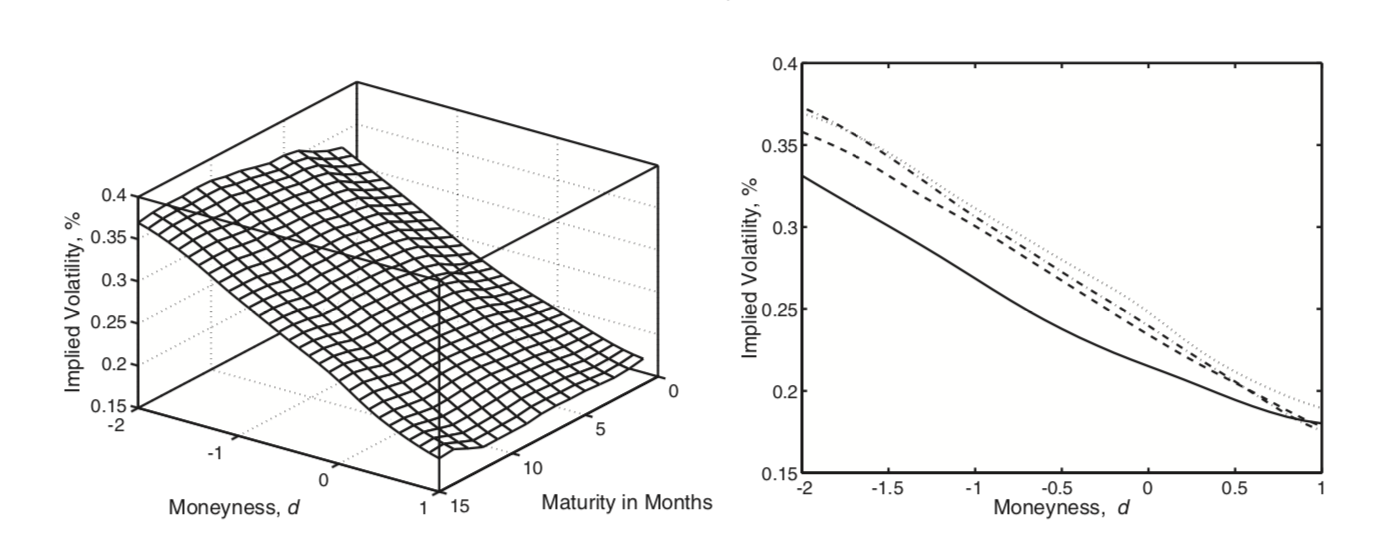
\includegraphics[width=1\linewidth]{img/implied_volatility.png}
\end{center}


\newpage
\section{Использование преобразования Фурье}
В 1999 Карр и Мадан показали \cite{FFT:paper}, что в случае, когда характеристическая функция логарифма спота известна, для вычисления цены колл-опциона можно использовать преобразование Фурье, что позволяет как ощутимо уменьшить время вычисления цены, так и сделать процесс интегрирования более устойчивым. Не останавливаясь на деталях, приведем формулы для вычислений. Пусть $S_t$~-- спот на момент $t$, $K$~-- страйк, $T$~-- дата погашения опциона, $q_t(s)$~-- риск-нейтральная мера спота на момент $t$, $C_T(k)$~-- цена опциона со страйком $K = e^k$. Положим
\[ s_t = \ln{S_t} \]
\[ k = \ln{K} \]
\[ \phi_T(u) = \mathbb{E}\left[ \exp{ius_T} \right] \text{~-- хар. функция } s_T=\ln{S_T}\]
\[ C_T(k) = \int\limits_k^\infty e^{-rT}(e^s - e^k)q_T(s)ds \]
\[ c_T(k) = e^{\alpha k}C_T(k),\,\, \alpha > 0 \]
\[ \psi_T(v) = \int\limits_{-\infty}^{+\infty} e^{ivk} c_T(k) dk\]
Тогда можно показать, что 
\[ \psi_T(v) = \frac{e^{-rT}\phi_T(v - (\alpha + 1)i)}{\alpha^2 + \alpha - v^2 + i(2\alpha + 1)v} \]
\[ C_T(k) = \frac{e^{-\alpha k}}{\pi} \int\limits_0^\infty e^{-vk} \psi_T(v) dv \]

Правильный выбор параметра $\alpha$ очень важен для корректности вычислений. Карр и Мадан рекомендуют в качестве верхней границы допустимых значений $\alpha$ брать 
\( \frac{1}{4} \, \underset{\alpha > 0}{\mathrm{sup}}(\alpha \,\, | \,\, \mathbb{E}[S_T^{\alpha+1}] < \infty) \). От себя автор добавит, что начинать поиск $\alpha$ следует с 1, проверяя, что на близких значениях моделируемые цены сохраняют смысл (например, возрастают/убывают в зависимости от типа опциона).


\newpage
\section{Калибровка моделей}
В этом разделе будут подробно рассмотрены полученные результаты по качеству калибровки параметров, скорости сходимости параметров к оптимальным, устойчивости откалиброваных параметров. 

\subsection{Постановка задачи калибровки}
В случае калибровки моделей ценообразования опционов процесс сводится к решению задачи оптимизации вида:
\[
f_\text{error}(M(p_1, ..., p_k, S, \bar K, T, r, q), P_\text{real}) \rightarrow \underset{p_1, ..., p_k}{\min}
\]
где $f_\text{error}(\cdot \, , \cdot)$~-- метрика ошибки приближения, $M$~-- модельная цена опционов,\\ $p_1$, ..., $p_k$~-- параметры модели, $S$~-- спот-цена, $\bar K$~-- набор страйков, $T$~-- время до погашения, $r$ и $q$~-- безрисковая процентная ставка и доходность, соответственно, $P_\text{real}$~-- рыночные цены опционов. В данной работе для оценки качества приближения использовалась метрика RMSE, т.е. \( f_\text{error}(\bar v_1, \bar v_2) = \sqrt{ \frac{1}{n} \sum\limits_{i = 1}^n{(\bar v_1^i - \bar v_2^i)^2} } \). 
\par
Для нахождения глобального минимума на области допустимых моделью параметров использовался алгоритм differential evolution\cite{DE:paper1}\cite{DE:paper2}. Стоит отдельно отметить, что использование быстрого преобразования Фурье\cite{FFT:paper} при моделировании цены опционов особенно хорошо сказывается при калибровке моделей с большим числом параметров, например, для модели Хестона это помогло сократить время оптимизации набора из 20 страйков более чем в 15 раз.

\newpage
\subsection{Качество калибровки}
\label{quality:label}
Приведем сравнение качества калибровки моделей по метрике RMSE для каждого рабочего дня в интервале с 20.6.2011 до 16.3.2012, итого для 187 дней. Для наглядности также приведены результаты для модели Блэка-Шоулза.

\begin{center}
  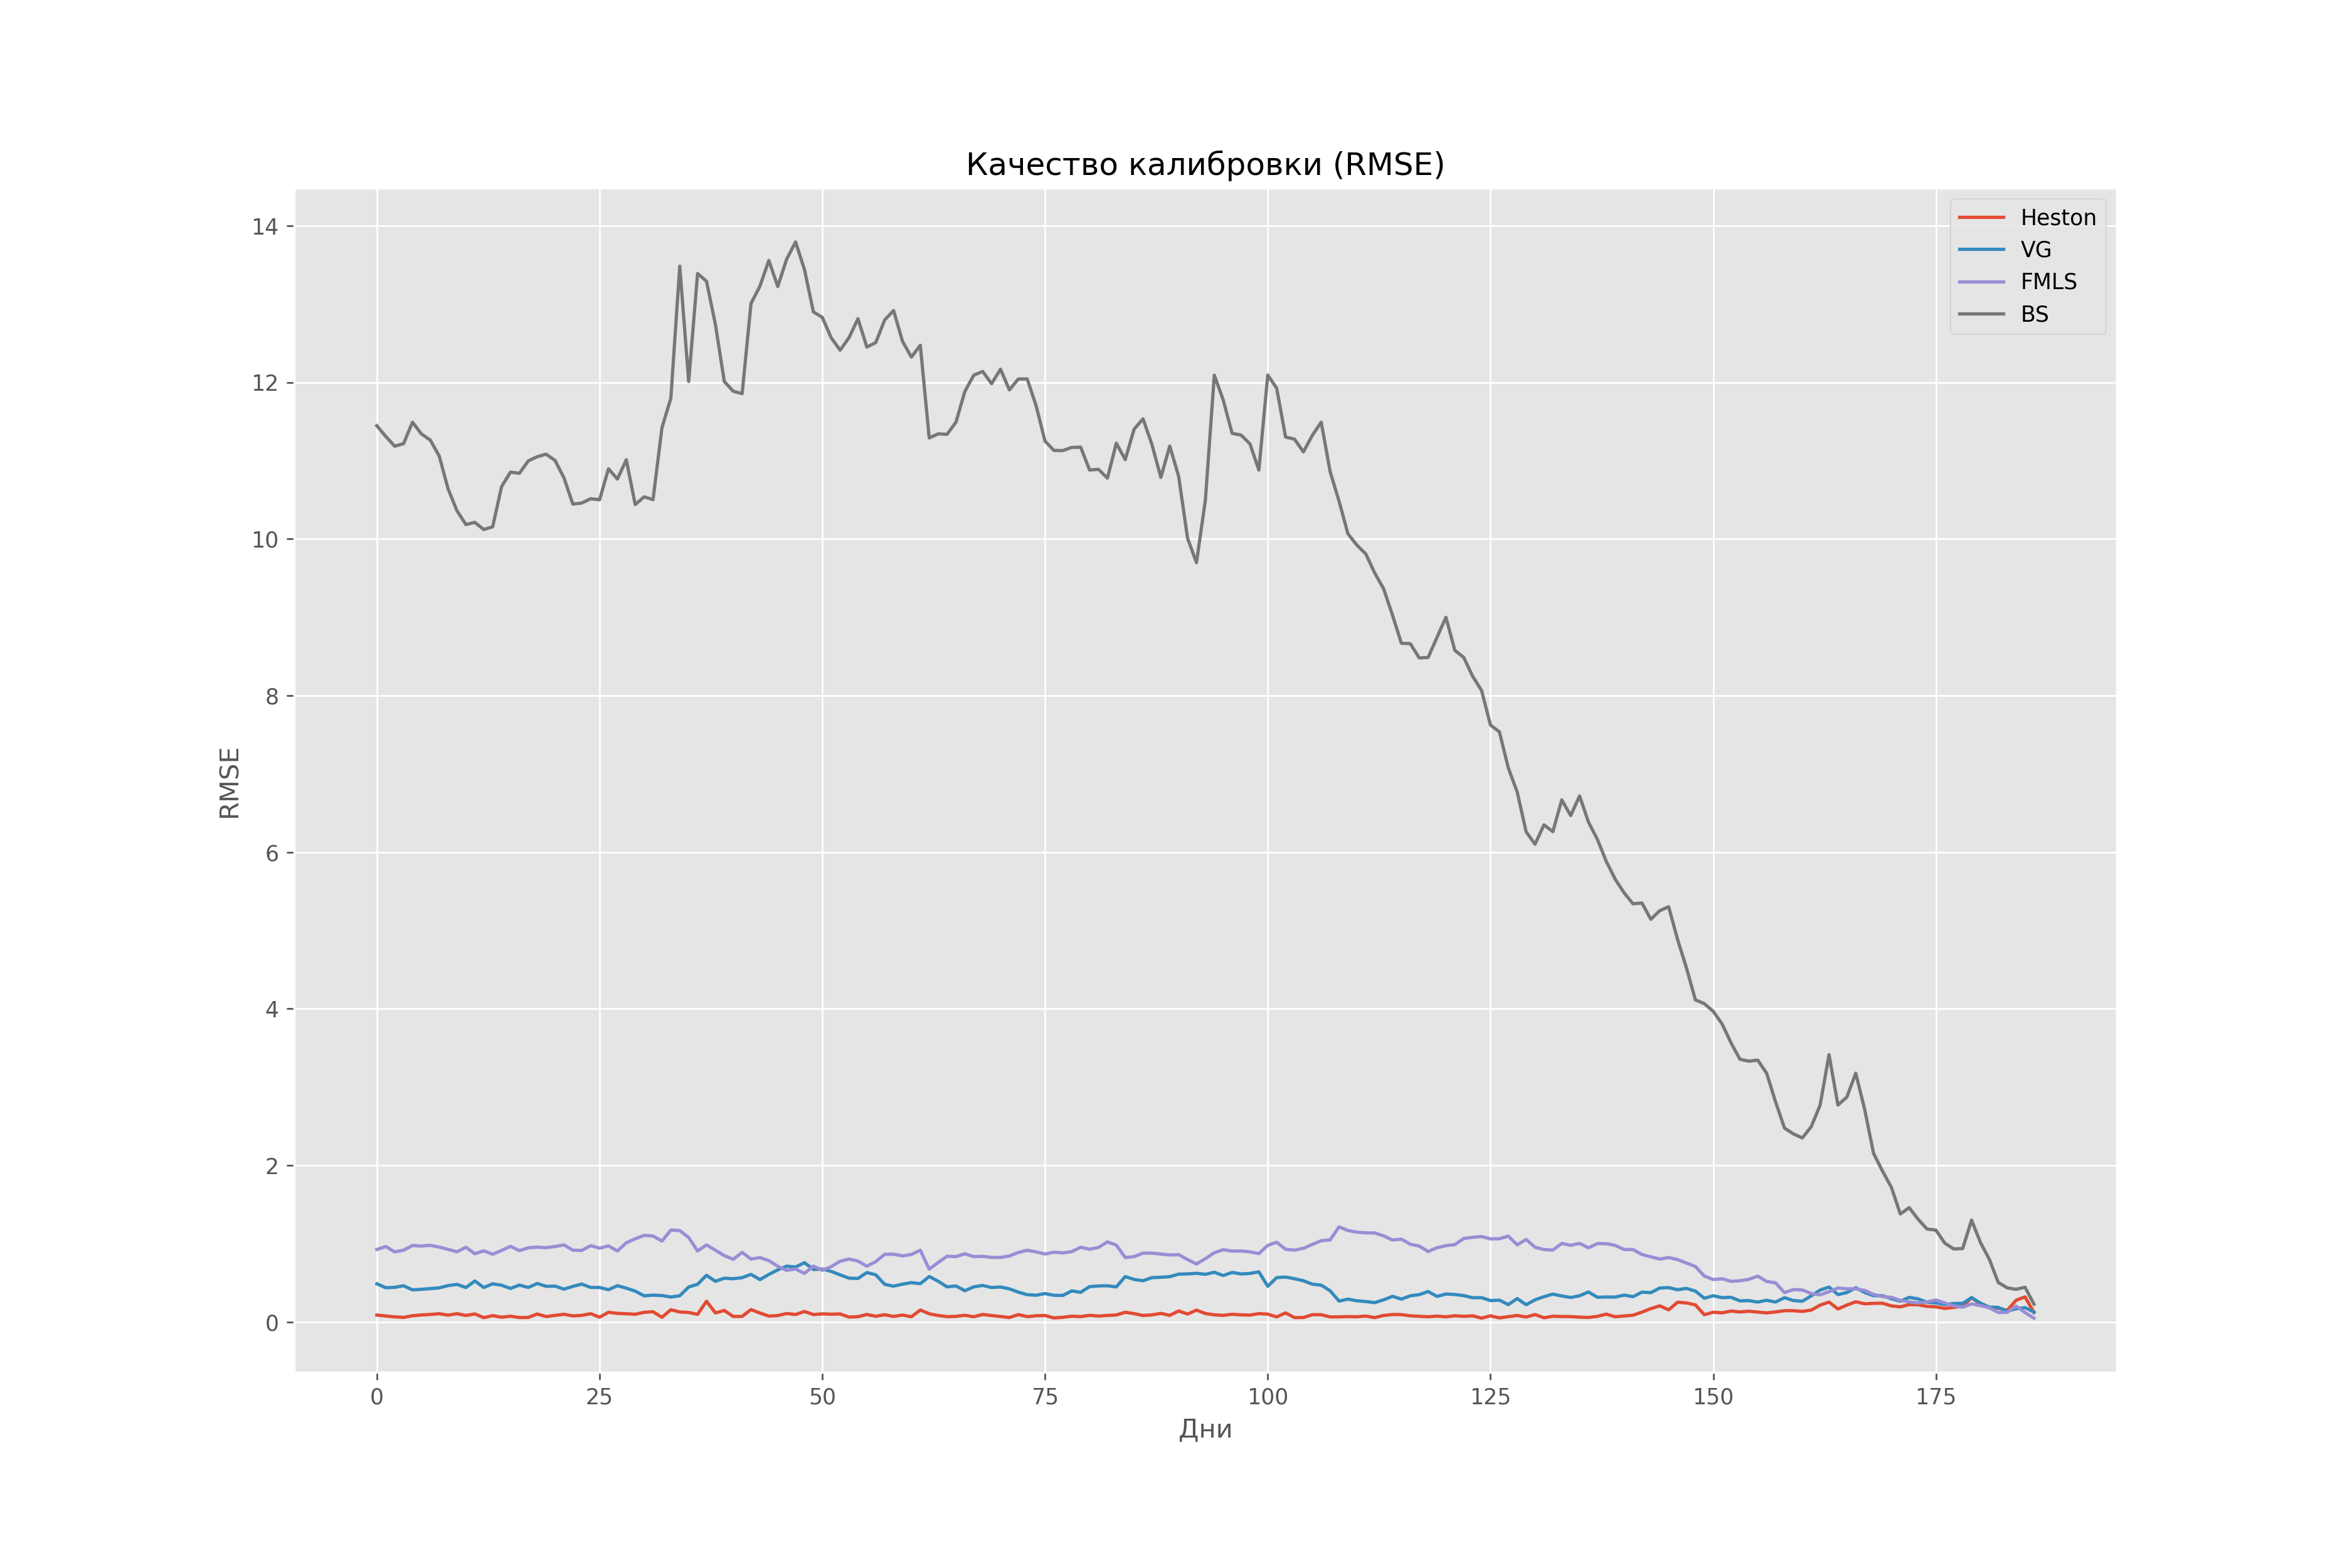
\includegraphics[width=1\linewidth]{img/RMSE_quality.png}
\end{center}

Хорошо видно, что модель Хестона подгоняется под реальные данные лучше VG и FMLS, выравниваются метрики примерно за неделю до экспирации. Модель же Блэка-Шоулза безнадежно отстала от наших трех моделей, лишний раз иллюстрируя свою непригодность. При этом стоит отметить, что значение спота составляло около 1200 на протяжении дней измерения, что означает, что все модели (кроме Блэка-Шоулза) достаточно хорошо калибруются, показывая среднюю ошибку порядка 0.1\% от значения спота.

\newpage
\subsection{Скорость калибровки}
Очевидно, что нет никакого смысла приводить абсолютные временные замеры. В качестве единицы отсчета возьмем среднее время калибровки модели Блэка-Шоулза на машине автора. Первая таблица показывает среднее время расчета цены K опционов с использованием FFT\cite{FFT:paper}. Вторая таблица приводит среднее время калибровки на реальных данных на K страйках, используя алгоритм differential evolution\cite{DE:paper1}.

\label{speed:label}

\begin{table}[h!]
  \begin{center}
    \caption{Средняя скорость расчета цены}
    \label{tab:table1}
    \begin{tabular}{c|c|c|c}
      \textbf{K} & \textbf{Heston} & \textbf{VG} & \textbf{FMLS}\\
      \hline
      1   & 4.4 & 2.78 & 2.67\\
      10  & 9.62 & 8.08 & 7.96\\
      25  & 12.5 & 11.37 & 11.44\\
      50  & 24.58 & 23.47 & 22.97\\
      100 & 39.63 & 40.52 & 37.02\\
      200 & 61.39 & 60.85 & 58.49\\
    \end{tabular}
  \end{center}
\end{table}

\begin{table}[h!]
  \begin{center}
    \caption{Средняя скорость калибровки}
    \label{tab:table2}
    \begin{tabular}{c|c|c|c}
      \textbf{K} & \textbf{Heston} & \textbf{VG} & \textbf{FMLS}\\
      \hline
      1   & 23 & 11 & 7 \\
      10  & 155 & 89 & 21\\
      25  & 245 & 128 & 29\\
      50  & 470 & 284 & 57\\
      100 & 865 & 488 & 102\\
      200 & 1126 & 730 & 156\\
    \end{tabular}
  \end{center}
\end{table}


\subsection{Устойчивость оптимальных параметров}
\label{stability:label}
\subsubsection{Устойчивость по вариации}
При прогнозе цен опционов на уже откалиброванных параметрах важно уделить внимание устойчивости~-- средним колебаниям ($ \sqrt{\mathbb{D}\xi}\;/\;\mathbb{E}|\xi| $) параметров при повторных калибровках. Оказалось, что модели VG и FMLS крайне устойчивы: вариация пренебрежимо мала по сравнению со значением параметра.

\begin{center}
  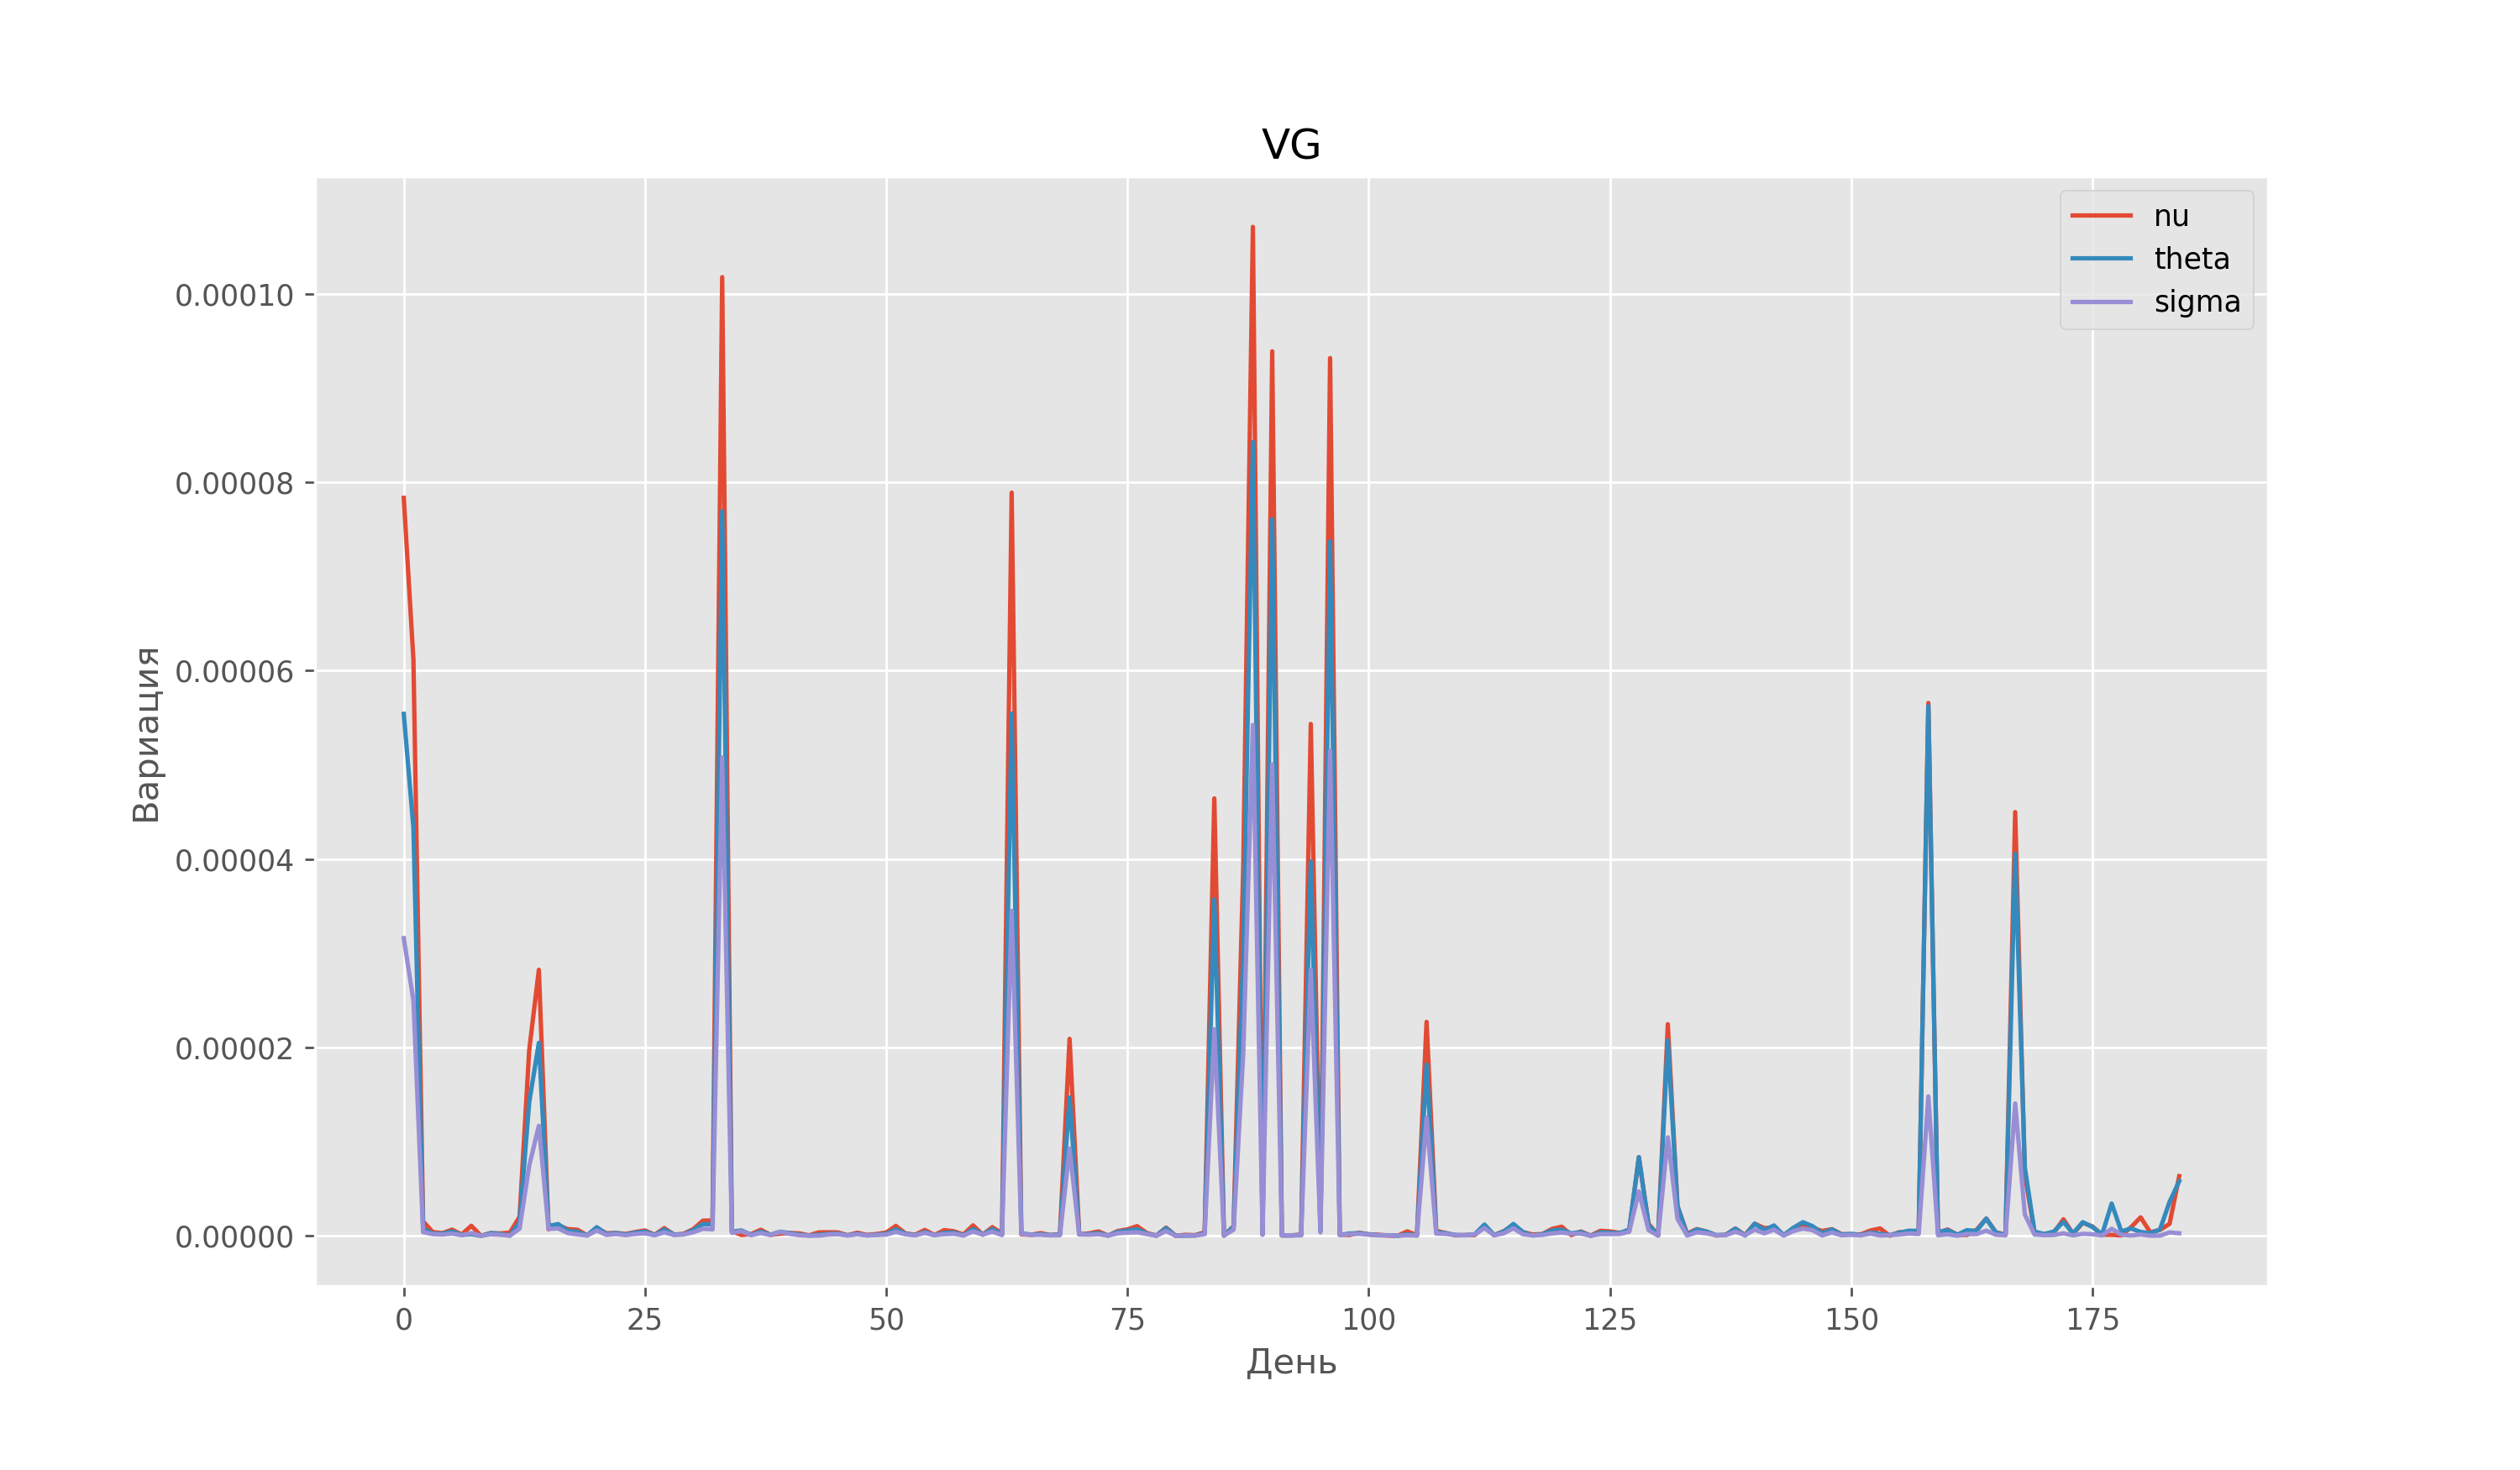
\includegraphics[width=1\linewidth]{img/vg_stable.png}
\end{center}

\begin{center}
  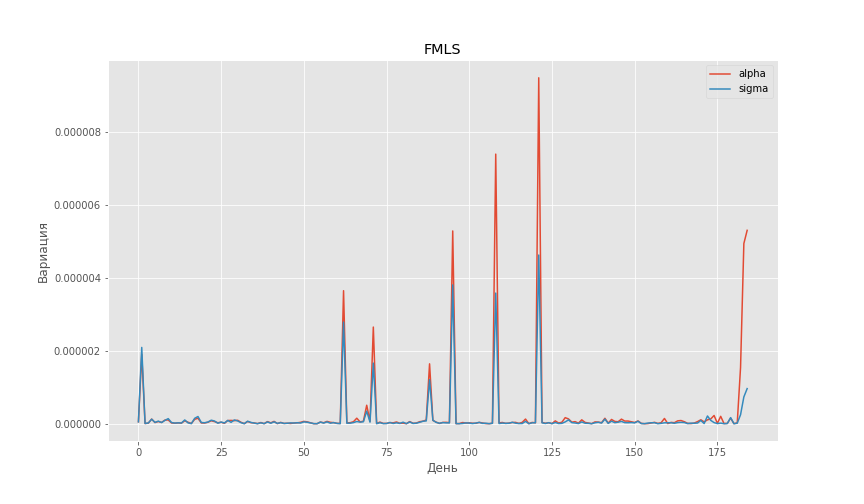
\includegraphics[width=1\linewidth]{img/ls_stable.png}
\end{center}


\newpage
Анализ же модели Хестона показывает, что устройчив лишь параметр $\rho$~-- корреляция винеровских процессов.
Безусловно, это необходимо учитывать при построении прогнозов с помощью откалиброванной модели. 

\begin{center}
  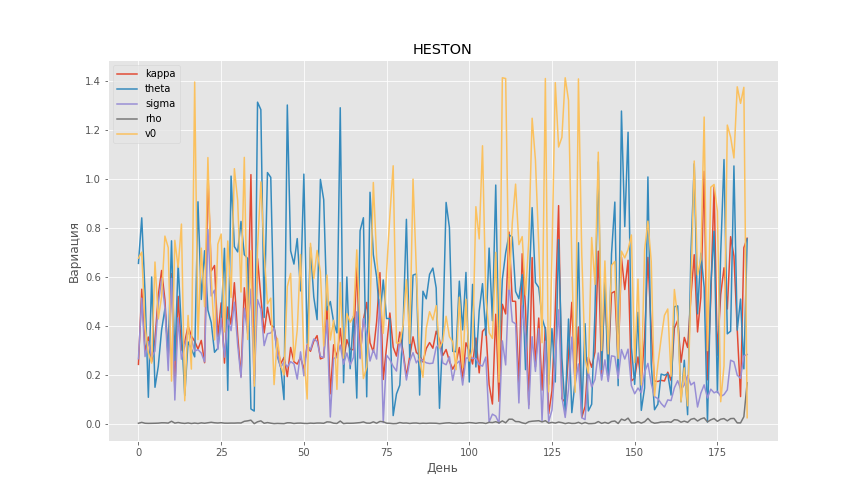
\includegraphics[width=1\linewidth]{img/heston_stable.png}
\end{center}

Отметим, что модель Блэка-Шоулза также очень устойчива (значение вариации показано без фактора $10^{-7}$)

\begin{center}
  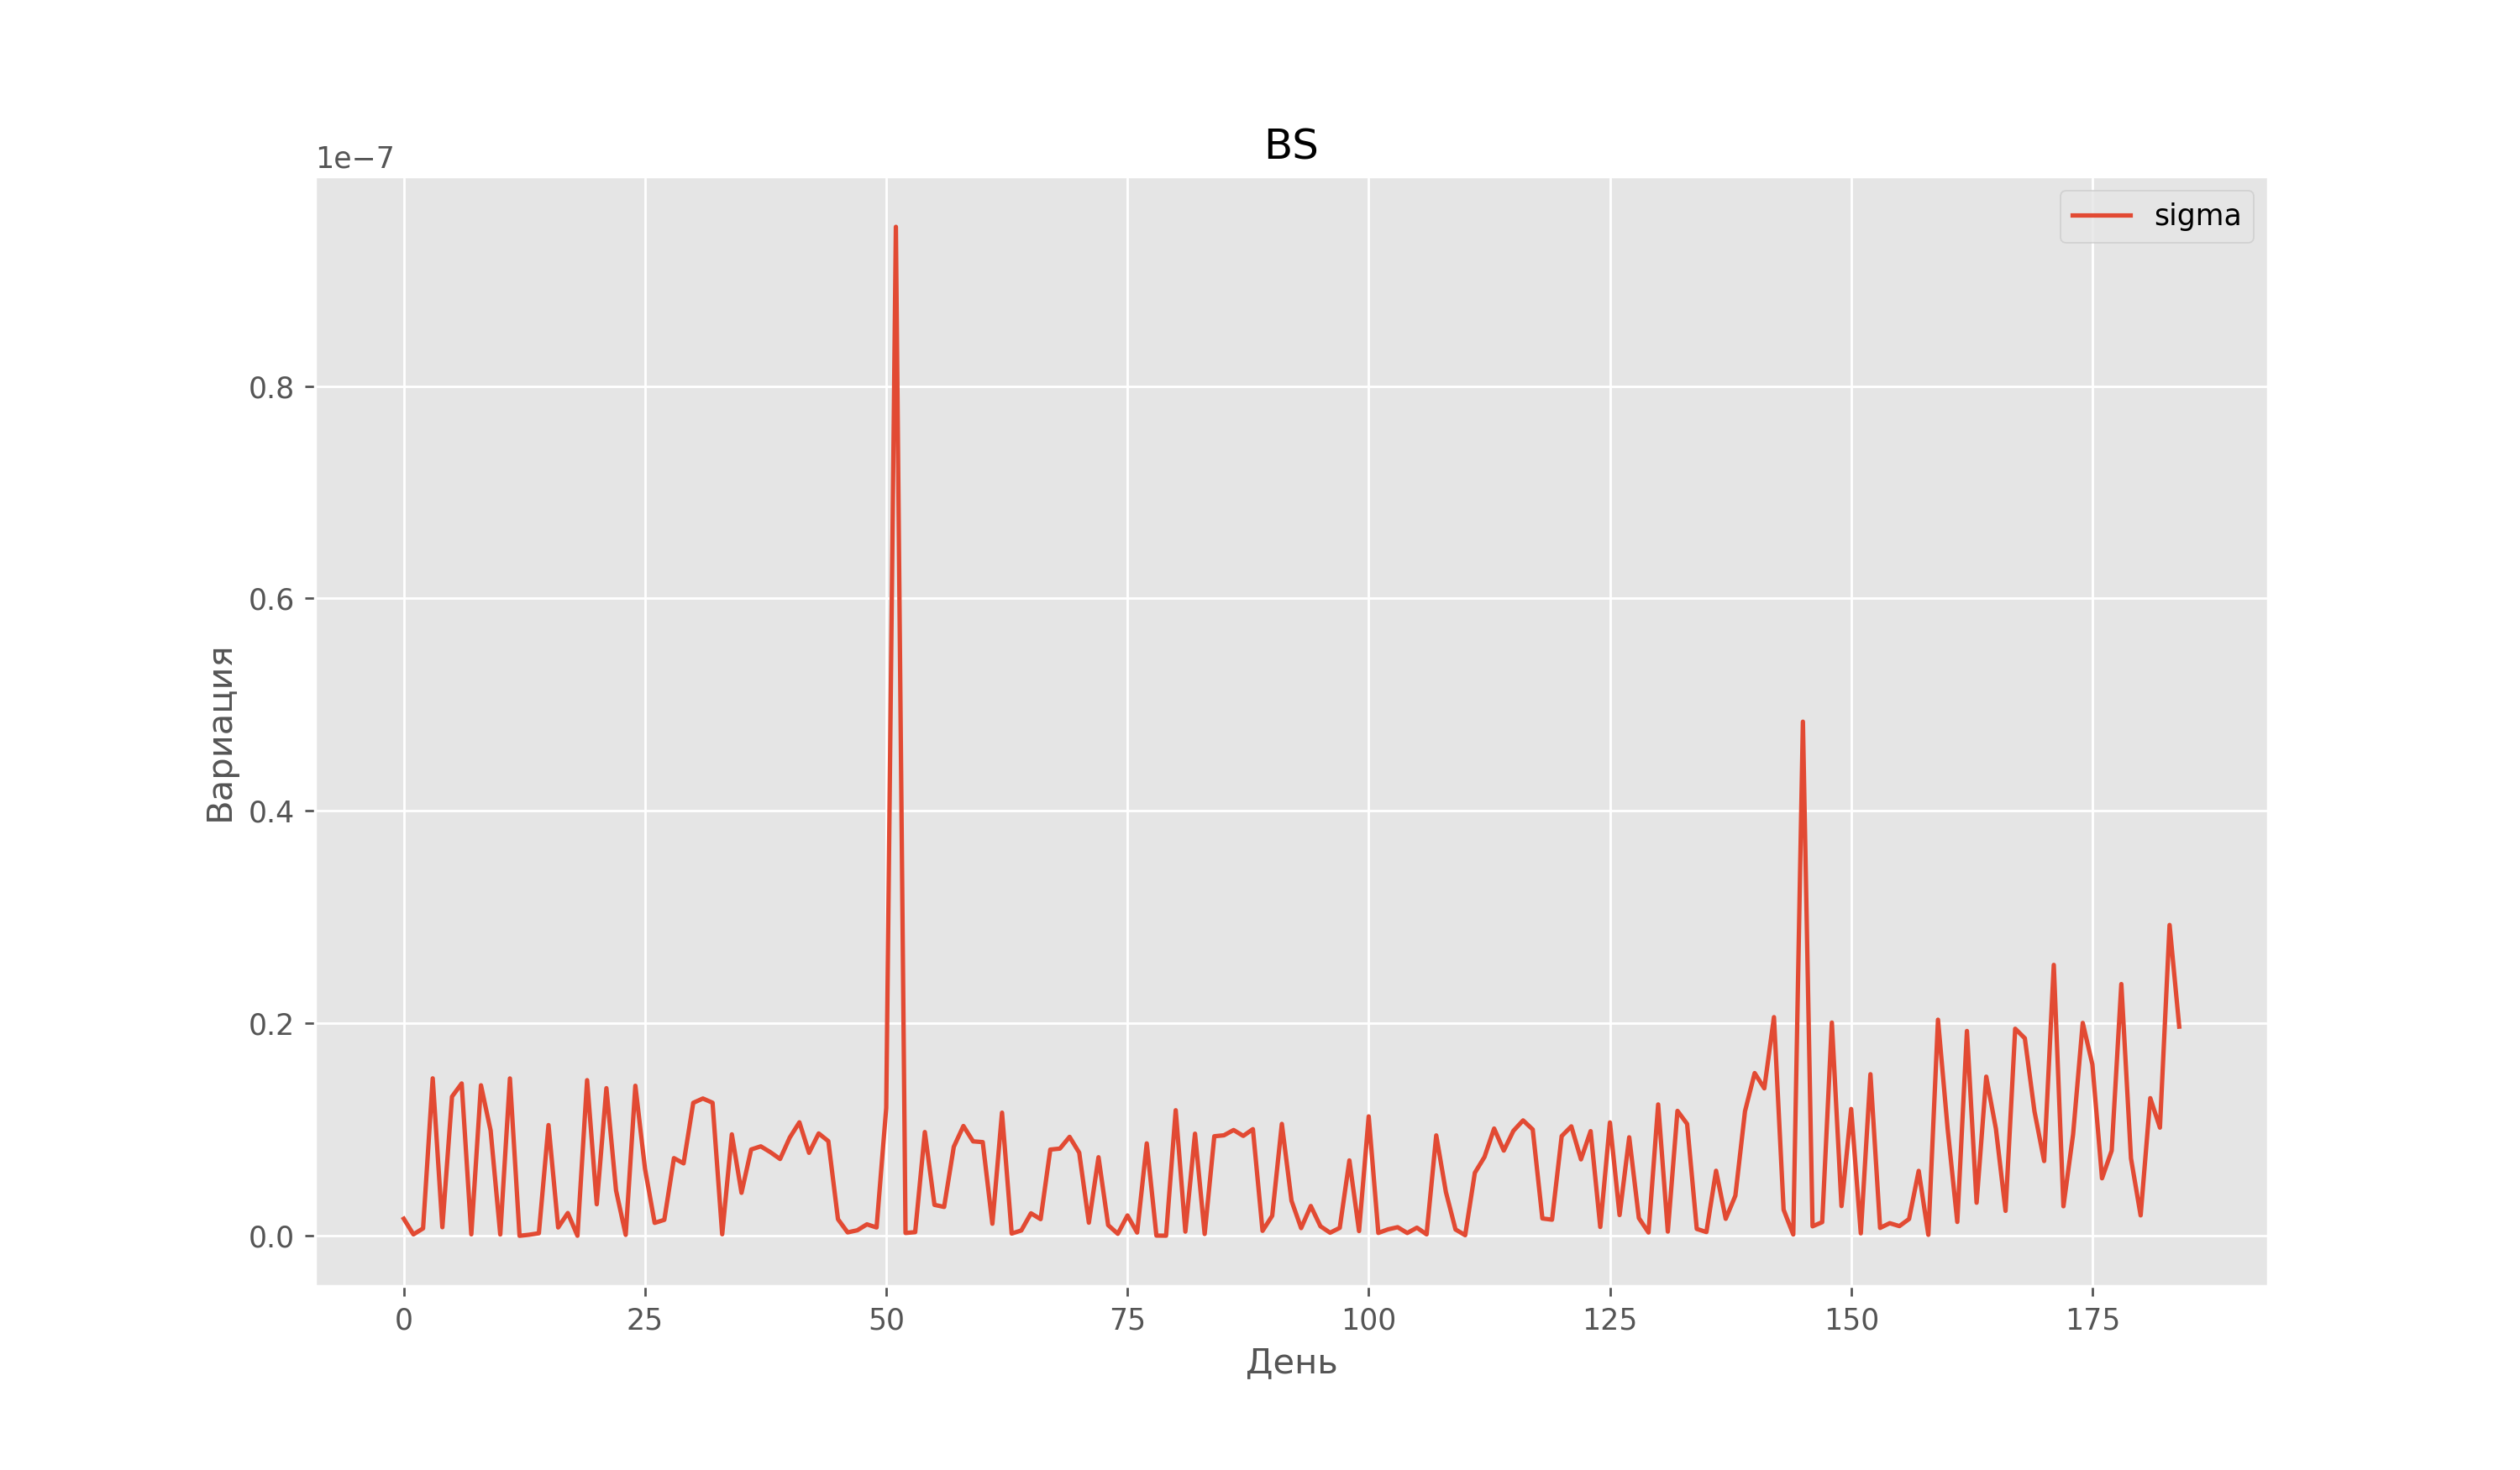
\includegraphics[width=1\linewidth, height=9cm]{img/bs_stable.png}
\end{center}

\newpage
\subsubsection{Устойчивость по времени}
Рассмотрим также устойчивость по времени~-- отношение значения параметра на следующем дне к предыдущему. Отметим, что на графике модели Хестона значения превосходящие 10, были обрезаны ввиду их сильного искажающего эффекта.

\begin{center}
  \includegraphics[width=1\linewidth, height=9cm]{img/vg_stable_rel.png}
\end{center}

\begin{center}
  \includegraphics[width=1\linewidth, height=9cm]{img/ls_stable_rel.png}
\end{center}

\begin{center}
  \includegraphics[width=1\linewidth, height=10cm]{img/heston_stable_rel.png}
\end{center}

Результаты приводят к аналогичным выводам~-- модели VG и FMLS достаточно устройчивы, параметры изменяются в среднем на 10-15\%. Модель Хестона же устойчивой считать никак нельзя.


\newpage
\section{Поиск оптимальных областей}
\label{VSK:label}
Для того чтобы дать рекомендации по использованию той или иной модели в зависимости от наблюдаемых цен, было проведено следующее:
\begin{enumerate}
\item Область параметров, полученных при калибровке модели VG на рыночных данных, была окружена параллелепипедом, внутри которого была построена сетка из 1024 точек. Таким образом были получены параметры, похожие на \lq\lq{}настоящие\rq\rq{}. Модель VG была выбрана в качестве стартовой, т.к. ее параметры имеют понятную интерпретацию ввиду того, что по ним можно явно получить волатильность (volatility), коэффициент скошенности (skewness), коэффициент эксцесса (kurtosis), см. \ref{VG:params}
\item По этим параметрам были построены модельные цены, опять же, близкие к реальным, на которых были откалиброваны модели Хестона и FMLS, на каждой из которых затем были откалиброваны две другие. Таким образом были проведены 6 калибровок, по 2 на каждую из моделей. Описанный процесс является симметричным в том смысле, что каждая из моделей была и калибрующей, и калибруемой для двух других.
\item Тогда для каждой точки из задающих исходные параметры VG имеем 6 метрик качества \( S_{m1, m2} \), где \( \text{m1} \not = \text{m2} \). Поставим в соответствие каждой модели m число \( S_m = \frac{\sum\limits_{m1 = m, m2 \not = m}{S_{m1, m2}}}{\sum{S_{m1, m2}}} \). Тогда модель с наименьшим значением $S_m$ является наилучшей.
\end{enumerate}

После проведения описанной процедуры были получено следующее:
\begin{itemize}
\item При значениях волатильности больше 0.2 и коэффициента скошенности меньше -1 модель FMLS стабильно превосходит остальные по качеству приближения, и это ожидаемо из построения процесса (см. \cite{LS:paper}). 
\item На оставшейся области модели Хестона и VG одинаково хороши (и значительно лучше, чем FMLS). 
\item Коэффициент эксцесса \footnote{Отметим, что под коэффициентом эксцесса с.в. $X$ здесь понимается величина \( \frac{\mathbb{E}[(X - \mathbb{E}X)^4]}{(\mathbb{E}[(X - \mathbb{E}X)^2])^2} - 3 \), т.о. рассматривались только распределения с \lq\lq{}толстыми\rq\rq{} хвостами}
 сам по себе почти не оказывает влияния на расположение областей предпочтимости моделей.
\end{itemize}

\begin{center}
  \includegraphics[width=.8\linewidth, height=10cm]{img/vol_skew_kurt.png}
\end{center}

\begin{center}
  \includegraphics[width=1\linewidth, height=10cm]{img/vol_skew_kurt_projections.png}
\end{center}


\newpage
\section{Прогнозирование цен}
\label{forecast:label}
\subsection{Долгосрочный прогноз}
В данном разделе показаны результаты прогнозирования с использованием моделей Хестона, VG  и FMLS по следующей схеме: прогноз строится каждые 30 рабочих дней, при этом параметры для прогноза берутся как оптимальные для начального дня в 30-дневном интервале. Тогда получаются следующие прогнозы (по оси X отложены дни, на второй и третьей картинках в группе отложены абсолютное отклонение текущего спота от спота в начальный день и само значение спота)

\begin{center}
  \includegraphics[width=1\linewidth, height=12cm]{img/forecast_0_30.png}
\end{center}

\begin{center}
  \includegraphics[width=1\linewidth, height=11cm]{img/forecast_30_30.png}
\end{center}
\begin{center}
  \includegraphics[width=1\linewidth, height=11cm]{img/forecast_60_30.png}
\end{center}

\begin{center}
  \includegraphics[width=1\linewidth, height=11cm]{img/forecast_90_30.png}
\end{center}
\begin{center}
  \includegraphics[width=1\linewidth, height=11cm]{img/forecast_120_30.png}
\end{center}

\begin{center}
  \includegraphics[width=1\linewidth, height=12cm]{img/forecast_150_30.png}
\end{center}

Сравнение показывает, что модели VG и FMLS дают почти неотличимые прогнозы, а прогноз по модели Хестона местами значительно отклоняется от двух других, показывая то лучшее значение RMSE, то худшее. Таким образом, нет возможности сказать, какая из моделей лучше подходит для посторения прогнозов.

Была также предпринята попытка предсказывать будущие параметры с использованием тренда за предыдущий интвервал, но прогнозы, постороенные с такой поправкой, получались в среднем хуже, так что эта идея была отброшена.


\newpage
\subsection{Краткосрочный прогноз}
Посторим теперь прогнозы на день вперед: модельными параметрами будем брать оптимальные параметры для предыдущего дня, цены которго считаем известными. Тогда имеем следующее:

\begin{center}
  \includegraphics[width=1\linewidth, height=14cm]{img/forecast_1_forward.png}
\end{center}

Видно, что в тех ситуациях, когда ошибки прогнозов вообще различимы, модель Хестона дает наилучшие результаты. Таким образом, можно дать рекомендацию по использованию модели Хестона для построения краткосрочных прогнозов.


\newpage
\section{Сравнение по AIC}
Сравним также модели по информационному критерию Акаике (AIC)\cite{AIC:paper}: \( \text{AIC} = 2k - 2\ln{L} \), где $k$~-- число параметров модели,  $L$~-- максимизированное значение функции правдоподобия. Отметим, что абсолютное значение AIC не имеет смысла, и наилучшей считается модель с наименьшим значением AIC. Можно показать, что в предположениях об одинаковой длине выборок $n$, нормальной и независимой распределенности ошибок модели $\varepsilon_i$, \( AIC = 2k +  n\ln{\sum\limits_{i = 1}^n}{\varepsilon_i^2}\)
\begin{center}
  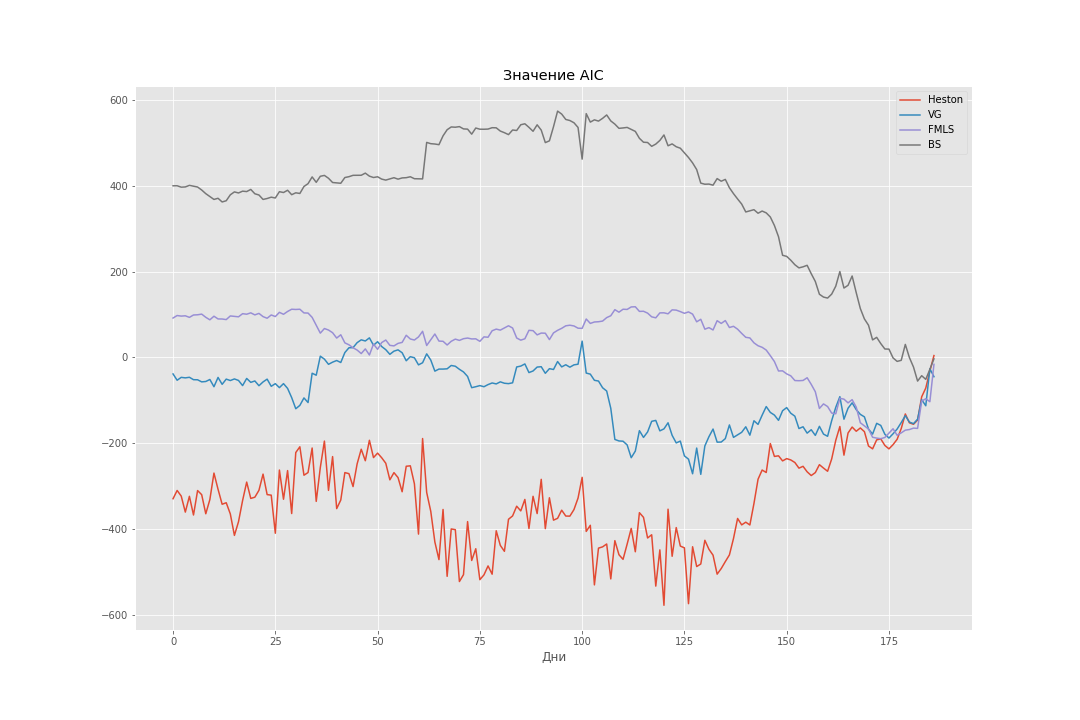
\includegraphics[width=1\linewidth]{img/AIC_187.png}
\end{center}

Результаты довольно ожидаемы: при больших выборках критерий Акаике отдает гораздо большее предпочтение качеству приближения, нежели сложности модели, и, таким образом, модель Хестона имеет заметно лучшее значение AIC, чем модели VG и FMLS.


\newpage
\section{Выводы}
Обобщая полученные в ходе работы результаты, выделим основные результаты:
\begin{itemize}
\item Была разработана методика (раздел \ref{VSK:label}) сравнения вероятностных моделей описания цены опциона, позволяющая определить наиболее подходящую модель на основе исторических данных о движении цены. В частности, в этом же разделе показано, что существует четкое разделение областей применимости моделей FMLS и VG/Хестона. При этом область, на которой оптимальны либо модель VG, либо Хестона, имеет примерно одинаковые показатели качества для обоих моделей. Таким образом, выбор между этими двумя моделями должен осуществляться по другим критериям.
\item Модель Хестона, хоть и дает наилучшие результаты при калибровке на рыночных данных (см. \ref{quality:label}), является недостаточно стабильной для долгосрочного прогнозирования ввиду слабой (особенно на фоне остальных моделей) устойчивости (см. \ref{stability:label}) откалиброванных параметров. В разделе \ref{forecast:label} показано, что модели VG и FMLS дают примерно одинаковые прогнозы, предсказание же по модели Хестона иногда заметно от них отклоняется. Возможно, что исскуственное ограничение множества допустимых параметров решит проблему неустойчивости параметров модели Хестона, позволив сохранить качество подгонки под реальные данные, но в таком случае остается открытым вопрос о границах такого отсечения.
\item Не менее важным ограничением модели Хестона является скорость калибровки: уже при небольшом наборе из 10 страйков процесс калибровки параметров модели Хестона занимает в 1.5-2 раза больше времени, чем калибровка VG, и на порядок, в 7-8 раз, больше, чем подгонка двух параметров FMLS (см. \ref{speed:label}). Отметим, что на сегодняшний день именно скорости расчетов отдается предпочтение, например, в биржевой торговле, где каждую минуту происходят тысячи заявок на покупку/продажу и котировки меняются исключительно быстро. В ситуации, когда скорость принятия решений играет решающее значение, модель Хестона не является применимой.
\end{itemize}


\newpage
\section{Заключение}
Подводя итог проделанной работе, хочется отметить следующее:
\begin{itemize}
\item Ввиду технических ограничений все калибровки проводились по 187 рабочим дням 2011 года. Уже после выполнения работы были получены данные за 91 рабочий день 2017/2018 года, при прогоне аналогичных тестов и метрик все выводы остались прежними. Безусловно, хотелось бы увеличить охват исследуемых дней~-- это остается для будущих работ.
\item В последующих работах стоит обратить внимание на более современные модели оценивания опционов, как, например, в работе Grzelak, L.A. \& Oosterlee, C.W. (2011), \lq\lq{}On the Heston Model with Stochastic Interest Rates\rq\rq{}, а также на методы, основанные на применении нейронных сетей.
\item Стоит пересмотреть построение системы точек VSK (см. \ref{VSK:label}) таким образом, чтобы эта система была более распределена по допустимой области. Например, этого можно было бы добиться, решая для каждой выбранной точки VSK обратную задачу по построению параметров \( \nu, \theta, \sigma \) модели VG, исходя из уравнений, указанных в разделе \ref{VG:params}.
\item Отдельным интересным направлением для изучения является выбор алгоритма глобальной оптимизации для калибровки параметров моделей. Выбор автора, алгоритм differential evolution\cite{DE:paper1}, был основан лишь на общей применимости алгоритма и на удовлетворительных результатах калибровки с его использованием.
\item \url{https://github.com/shvimas/diploma.git}~-- репозиторий со всем необходимым для воспроизведения результатов автора. В том числе в нем реализованы все три используемые в работе модели (Хестона, VG и FMLS), стороннюю реализацию которых автор не смог найти для языка Python (для моделей Хестона и VG есть реализация на R, но она оставляет желать лучшего).
\end{itemize}



\newpage
\begin{thebibliography}{00}
\bibitem{Heston:paper} Steven L. Heston (1993)
\emph{A Closed-Form Solution for Options with Stochastic Volatility with Applications to Bond and Currency Options}

\bibitem{LS:paper} Peter Carr, Liuren Wu (2003)
\emph{The Finite Moment Log Stable Process and Option Pricing}

\bibitem{VG:paper} Dilip B. Madan, Peter P. Carr, Eric C. Chang (1998)
\emph{The Variance Gamma Process and Option Pricing}

\bibitem{FFT:paper} Peter Carr, Dilip B. Madan (1999)
\emph{Option valuation using the fast Fourier transform}

\bibitem{DE:paper1} Rainer Storn, Kenneth Price (1997)
\emph{Differential Evolution — A Simple and Efficient Heuristic for Global Optimization over Continuous Spaces.}

\bibitem{DE:paper2} K. Price, R. Storn, J. Lampinen (2005)
\emph{Differential Evolution: A Practical Approach to Global Optimization}

\bibitem{AIC:paper} Akaike, H. (1974)
\emph{A new look at the statistical model identification}

\bibitem{Levy:paper} Gennady Samorodnitsky, Murad S. Taqqu (1994)
\emph{Levy Measures of Infinitely Divisible Random Vectors and Slepian Inequalities}

\end{thebibliography}

\end{document}